\documentclass{article}

\usepackage{graphicx}
\usepackage{tikz}
\usepackage{tikzsymbols}
\usetikzlibrary{calc,patterns,shapes.geometric}
\pagestyle{empty}
\usepackage[margin=0pt]{geometry}
\geometry{papersize={14in,12in}}

\def\centerarc[#1](#2)(#3:#4:#5){\draw[#1] ($(#2)+({#5*cos(#3)},{#5*sin(#3)})$) arc (#3:#4:#5);}

\begin{document}
	\begin{figure}
		\centering
		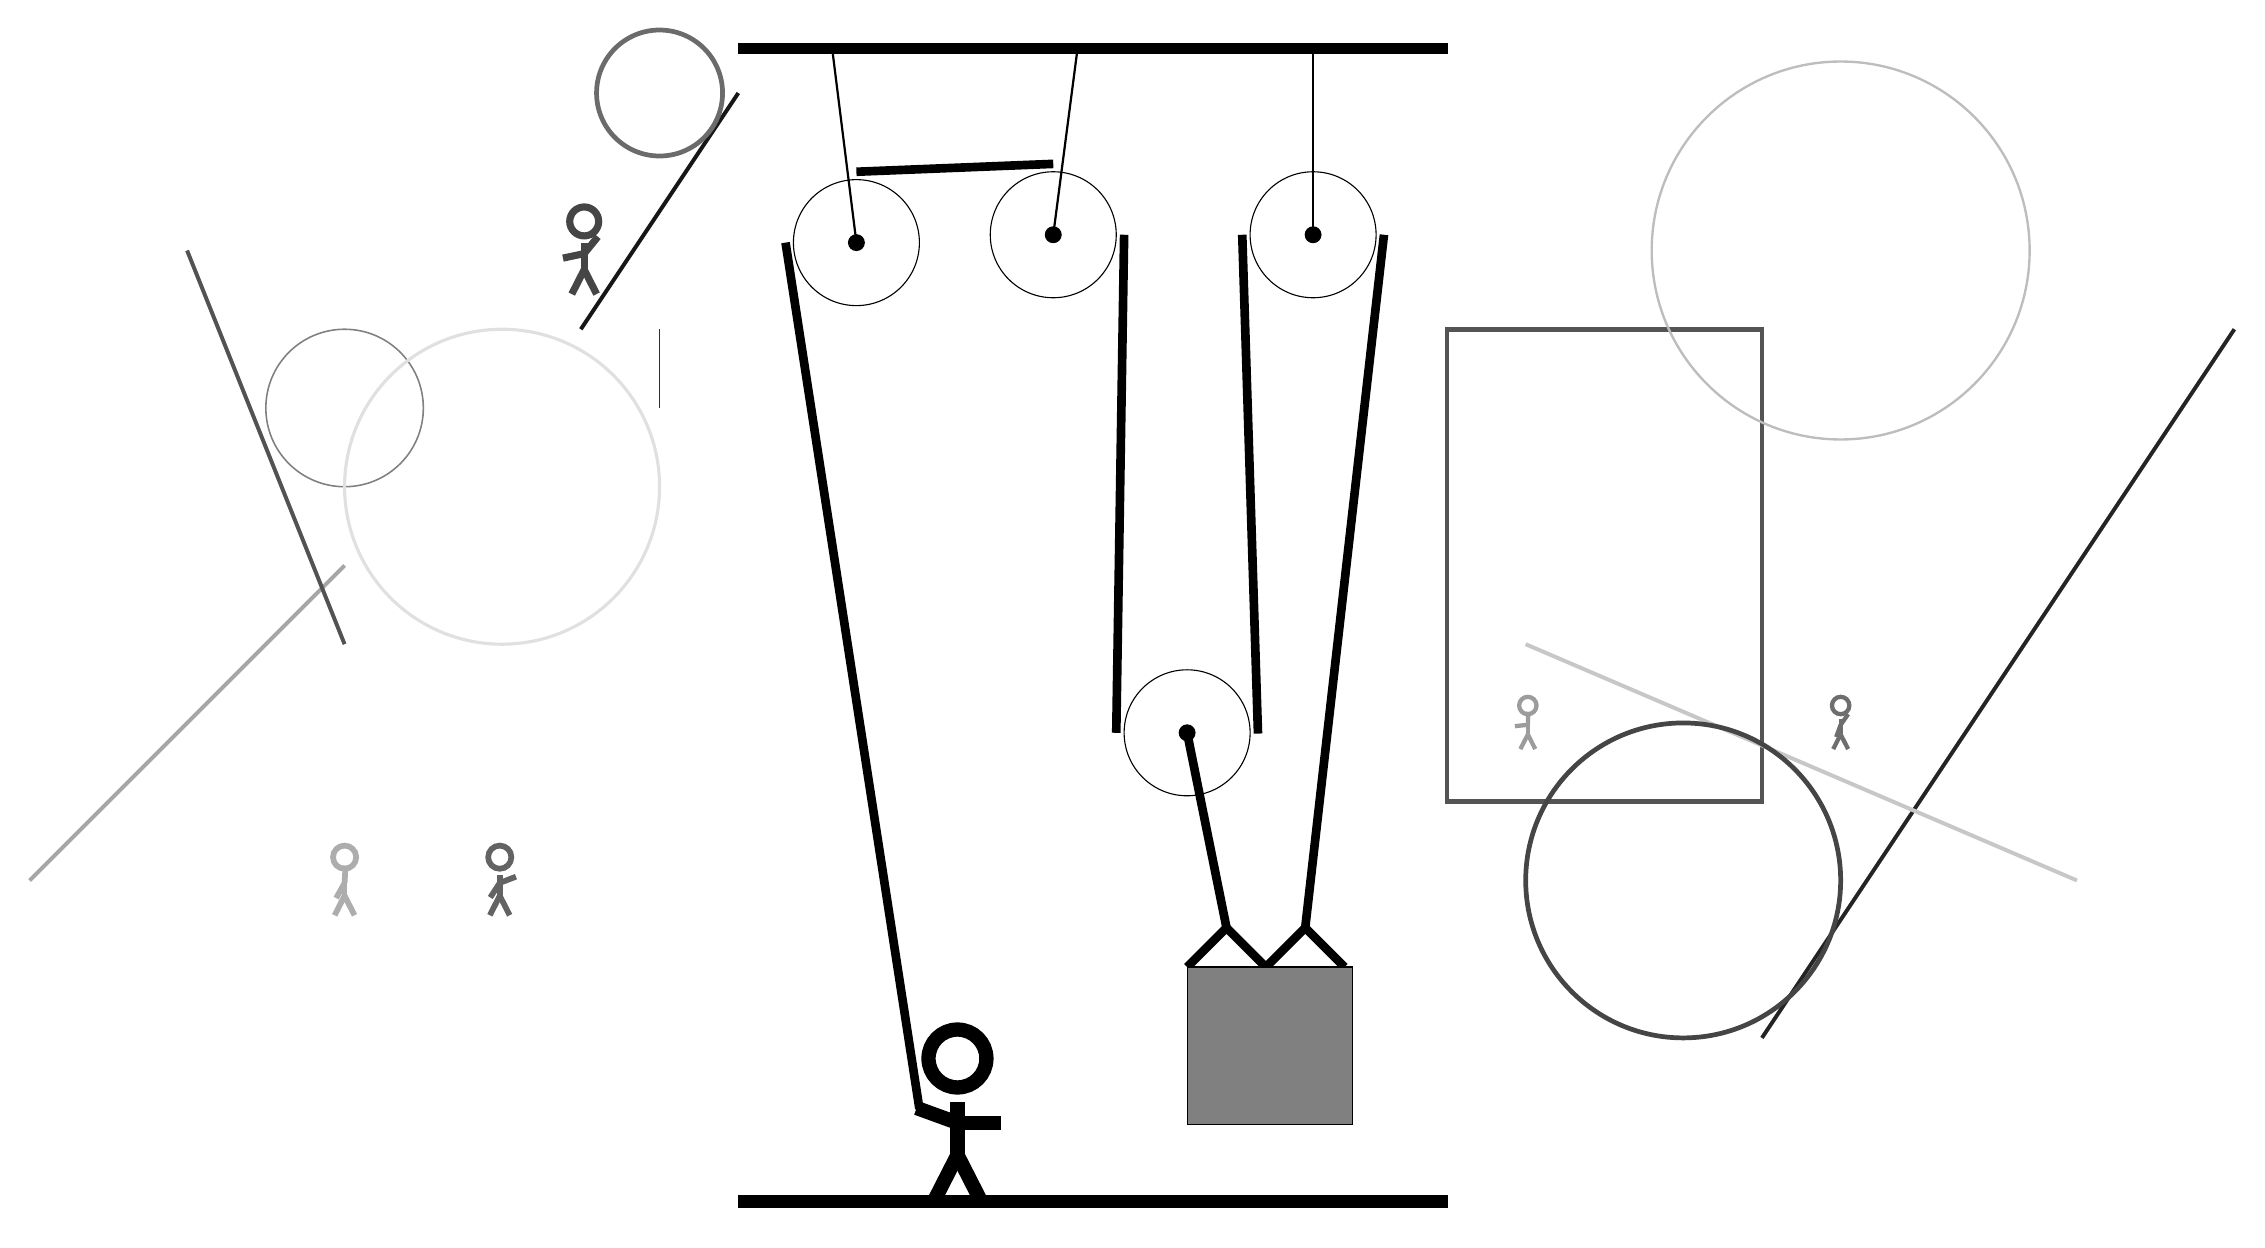
\begin{tikzpicture}
			%%%%% START %%%%%
			
			\draw[fill=black] (-3, 11.5) rectangle (6, 11.625);
			
			\draw (1, 9.2) circle (0.8);
			\draw[fill=black] (1, 9.2) circle (0.1);
			\draw[thick] (1, 9.2) -- (1.3, 11.5);
			
			\draw (4.3, 9.2) circle (0.8);
			\draw[fill=black] (4.3, 9.2) circle (0.1);
			\draw[thick] (4.3, 9.2) -- (4.3, 11.5);
			
			\draw (2.7, 2.875) circle (0.8);
			\draw[fill=black] (2.7, 2.875) circle (0.1);
			
			\draw[line width=0.6mm, color=black!67] (6, 8) rectangle (10, 2);
			
			\draw[line width=0.2mm, color=black!81] (-4, 7) rectangle (-4, 8);
			\draw[line width=0.5mm, color=black!91](-5, 8) -- (-3, 11);
			\node[line width=0.6mm, color=black!61] at (-6, 1) {\Strichmaxerl[4][57][21]};
			\draw [line width=0.2mm, color=black!50](-8, 7) circle (1.0);
			\node[line width=0.6mm, color=black!32] at (-8, 1) {\Strichmaxerl[4][61][87]};
			\draw [line width=0.4mm, color=black!12](-6, 6) circle (2.0);
			\node[line width=0.7mm, color=black!39] at (7, 3) {\Strichmaxerl[3][6][88]};
			\draw [line width=0.3mm, color=black!26](11, 9) circle (2.4);
			\draw[line width=0.5mm, color=black!35](-8, 5) -- (-12, 1);
			\draw [line width=0.6mm, color=black!58](-4, 11) circle (0.8);
			
			\draw[line width=0.5mm, color=black!86](10, -1) -- (16, 8);
			\draw[line width=0.5mm, color=black!22](7, 4) -- (14, 1);
			
			\node[line width=0.7mm, color=black!73] at (-5, 9) {\Strichmaxerl[5][12][51]};
			\draw [line width=0.6mm, color=black!73](9, 1) circle (2.0);
			\node[line width=0.7mm, color=black!57] at (11, 3) {\Strichmaxerl[3][70][55]};
			
			\draw[line width=0.5mm, color=black!68](-8, 4) -- (-10, 9);
			
			\draw[line width=1.1mm]  (2.7, -0.1) -- (3.2, 0.4) -- (3.7, -0.1) -- (4.2, 0.4) -- (4.7, -0.1);
			\draw[fill=black!50] (2.7, -0.1) rectangle (4.8, -2.1);
			
			\draw (-1.5, 9.1) circle (0.8);
			\draw[fill=black] (-1.5, 9.1) circle (0.1);
			\draw[thick] (-1.5, 9.1) -- (-1.8, 11.5);
			
			\draw[line width=1.1mm](-0.7, -1.9) --  (-2.4, 9.1);
			\centerarc[line width=1.1mm](-1.5, 9.1)(90:180:0.9);
			\draw[line width=1.1mm](-1.5, 10.0) -- (1, 10.1);
			\centerarc[line width=1.1mm](1, 9.2)(0:90:0.9);
			\draw[line width=1.1mm](1.9, 9.2) -- (1.8, 2.875);
			\centerarc[line width=1.1mm](2.7, 2.875)(180:370:0.9);
			\draw[line width=1.1mm] (3.6, 2.865) -- (3.4, 9.2);
			\centerarc[line width=1.1mm](4.3, 9.2)(0:180:0.9);
			\draw[line width=1.1mm](4.2, 0.4) -- (5.2, 9.2);
			\draw[line width=1.1mm] (3.2, 0.4) -- (2.7, 2.875);
			
			\node at (-0.2, -2) {\Strichmaxerl[10][-20][0]};
			
			\draw[fill=black] (-3, -3) rectangle (6, -3.15);
			
			%%%%% END %%%%%
		\end{tikzpicture}
	\end{figure}	
\end{document}